\documentclass{beamer}
\mode <presentation>
{
    \usetheme{boxes}
    \usecolortheme{crane}
    \setbeamercovered{transparent}
}

\usepackage[absolute,overlay]{textpos}
\usepackage{pgf,pgfarrows,pgfnodes}
\usepackage[english]{babel}
\usepackage{lmodern}
\usepackage{newcent}
\usepackage{amsmath}
% math extension - one probably wants to use symbols like '[' (written as '$[$')
\usepackage{ucs}
%\usepackage[utf8]{inputenc}
%\usefonttheme{structuresmallcapsserif}

% utf8x does not work with xetex
\usepackage[utf8x]{inputenc}

\usepackage[normalem]{ulem}


\setlength{\TPHorizModule}{1mm}
\setlength{\TPVertModule}{1mm}
\newcommand{\WorkInProgress}{%
\begin{textblock}{14}(120.0,75.7)

\includegraphics[height=0.7cm]{./pics/workinprogress.jpg}
\end{textblock}
  }

%\setbeamercolor{background canvas}{bg=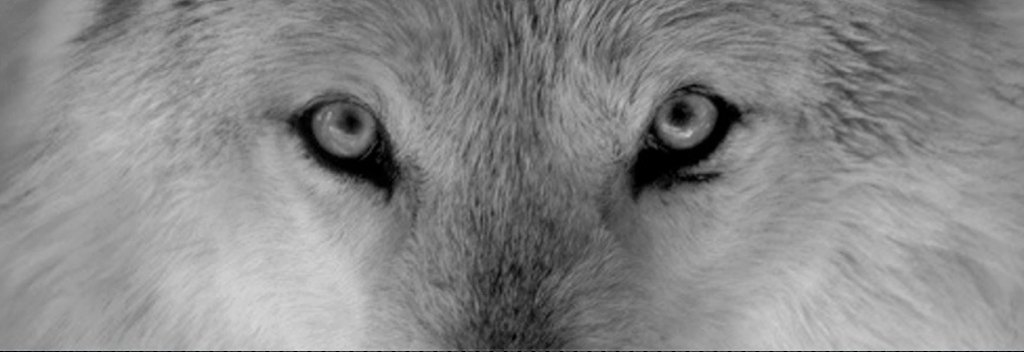
\includegraphics[width=\textwidth]{./pics/wolf.png}}

\title{Assets management with~FusionInventory~and~GLPI}
\author{\href{http://www.FusionInventory.org}{FusionInventory.org}}
\subject{Assets management with FusionInventory and GLPI}
\keywords{Assets management, Inventory, FusionInventory, GLPI}

\date{July 2011}
%\titlegraphic{GLPI}
%subtitle{
\includegraphics[width=1.2cm]{./pics/fusioninventory-logo.png}}
\institute{
\includegraphics[height=4.2cm]{./pics/rmll2011.jpg}}

\titlegraphic{}
%subtitle{
\includegraphics[width=1.2cm]{./pics/fusioninventory-logo.png}}
%\institute{
\includegraphics[height=4.2cm]{./pics/fusioninventory-logo.pdf}}
\author{ David Durieux \texttt{<d.durieux@siprossii.com>} \\
Gonéri Le Bouder \texttt{<goneri@teclib.com>}}
\logo{
\includegraphics[height=0.7cm]{./pics/fusioninventory-logo.pdf}}

\AtBeginSection[] % Do nothing for \section*
{
    \begin{frame}<beamer>
        \frametitle{Outline}
        \tableofcontents[currentsection]
    \end{frame}
}

%%%%%%%%%%%%%%%%%%%%%%%%%%%%%%%%%%%%%%%%%%%%%%%
%%%%%%%%%%%%%%%%%%%%%%%%%%%%%%%%%%%%%%%%%%%%%%%
\begin{document}

\frame[plain]{\titlepage}

\begin{frame}
    \frametitle{Who}

    \textbf{We are Legion!}
    \begin{center}
    
\includegraphics[height=3.5cm]{./pics/sparta.jpg}
    \end{center}

    \begin{itemize}
    \item about 10 core developers involved in the project
    \item active community of contributors
    \item 2 companies involved
    \end{itemize}

    \pause
    \bf{We are looking for people to JOIN US!}
\end{frame}


\begin{frame}
    \frametitle{About us: David Durieux}

    \begin{block}{IT management consultant}
        \begin{itemize}
        \item GLPI core-developer
        \item FusionInventory project co-leader
        \item Work at siprossii, Lyon area, France
        \end{itemize}
    \end{block}

\end{frame}



\begin{frame}
    \frametitle{About us: Gonéri Le Bouder}


    \begin{block}{Free software enthusiast}
        \begin{itemize}
        \item Debian Developer
        \item Perl Monger
        \item Former OCS Inventory developer
        \item FusionInventory project co-leader
        \item Work at TECLIB', Paris, France
        \end{itemize}
    \end{block}

\end{frame}

\begin{frame}
    \frametitle{The project workflow}
    %%-------------------------------------------------------------------
    %%\logo{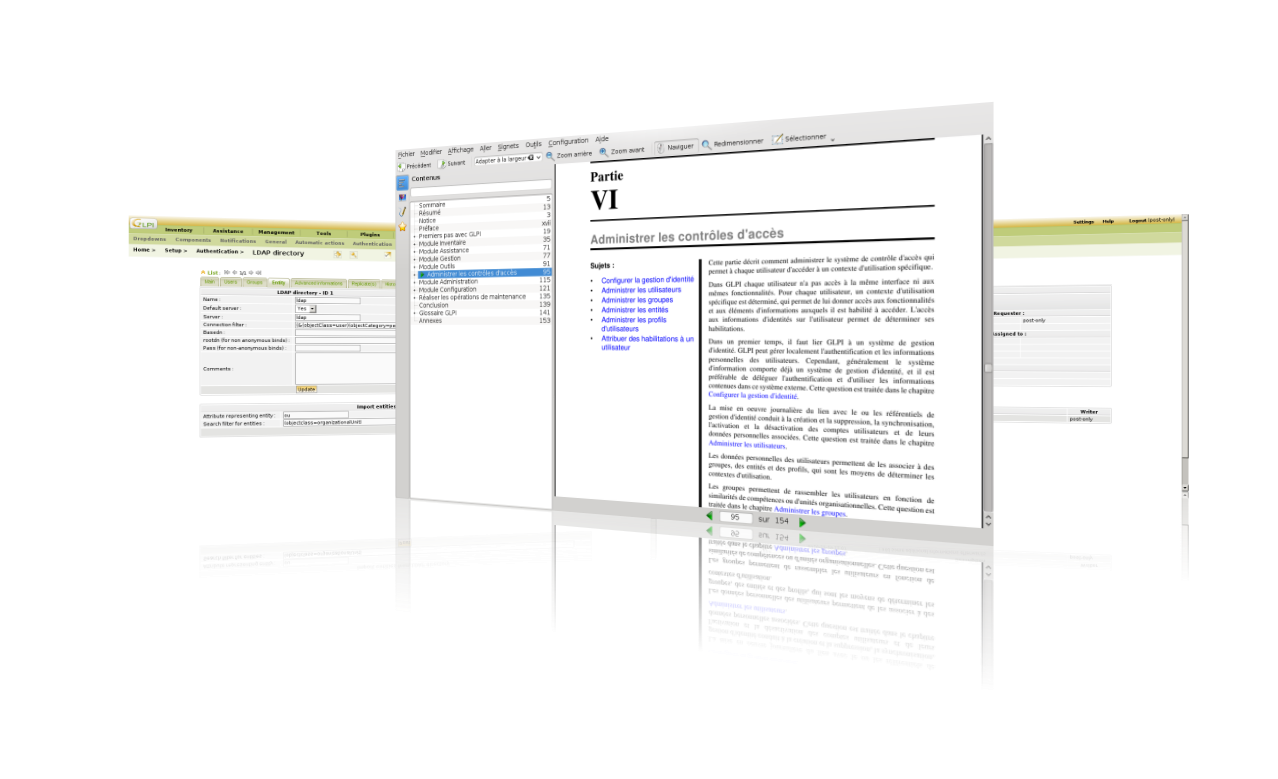
\includegraphics[height=3.5cm]{./pics/glpi-doc.png}}
    FusionInventory is a community-driven project.

    \begin{itemize}
        \item active mailing lists
        \item IRC: \#FusionInventory on FreeNode
        \item public Forge, Git repositories, etc
    \end{itemize}
\end{frame}


\section{Overview}


\begin{frame}
    \frametitle{Global overview}


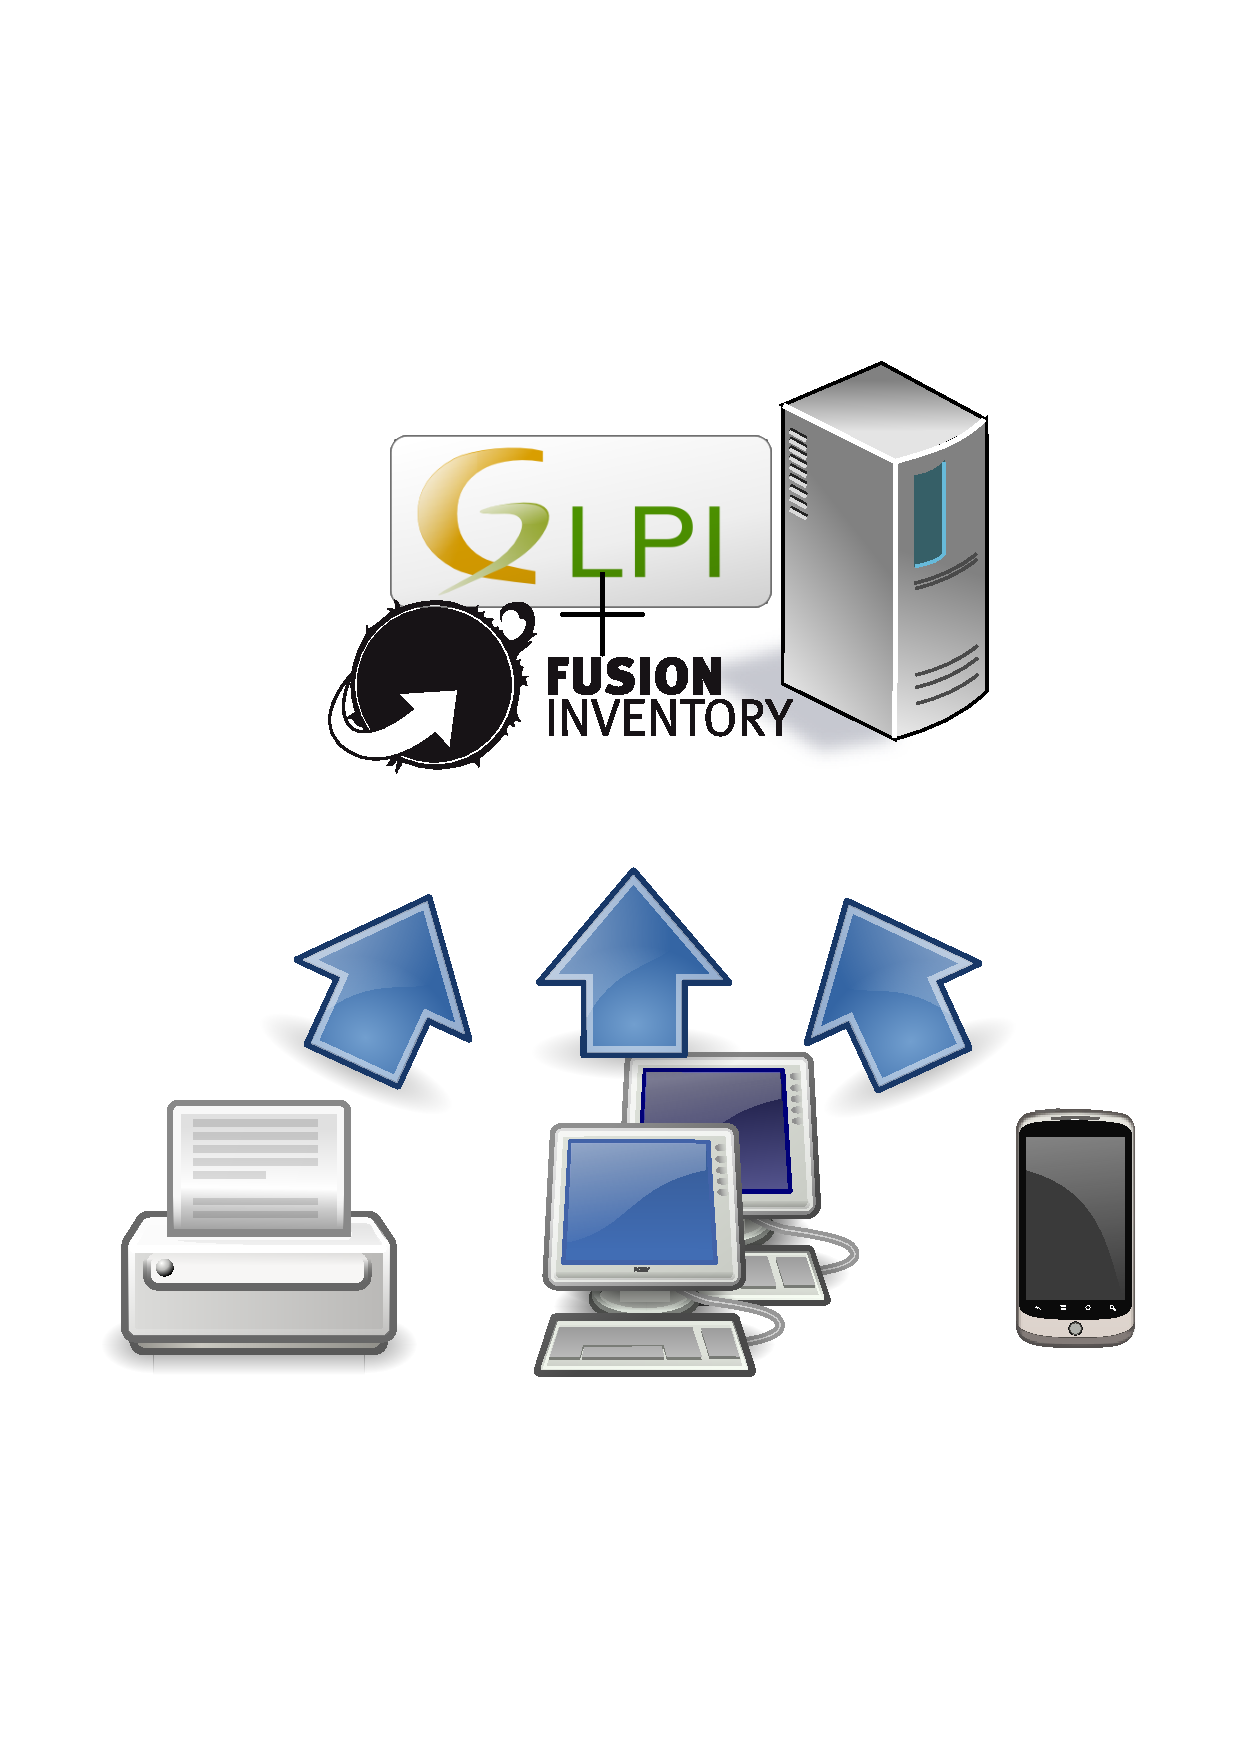
\includegraphics[height=9.5cm]{pics/basic_arch.pdf}

\end{frame}

%%
%\begin{frame}
%    \frametitle{Agent history}
%
%    \begin{center}
%    
\includegraphics[height=3.5cm]{./pics/agent-smith.jpg}
%    \end{center}
%
%
%    \begin{itemize}
%        \item a fork of OCS Inventory UNIX agent by its author
%        \item started 5 years ago
%        \item GPLv2
%    \end{itemize}
%\end{frame}

%\begin{frame}
%    \begin{center}
%    
\includegraphics[height=4.0cm]{pics/Perl_Foundation.pdf}
%    \end{center}
%    \frametitle{use Perl Luke!}
%
%    We choose to use Perl on the agent side.
%    \begin{itemize}
%        \item portable
%        \item reliable
%        \item versatile
%        \item stable API
%    \end{itemize}
%\end{frame}

%\begin{frame}
%    \frametitle{Agent pull}
%
%    \begin{center}
%
%%    
\includegraphics[height=5.0cm]{pics/kung-fu-panda.jpg}
%
%    \end{center}
%
%\end{frame}

\begin{frame}
    \frametitle{Agent pull / Server push}

    \begin{itemize}
    \item Connection are always created by the agent.
    \item A "push" option allow the server to contact the agent: just a trigger that awake the agent.
    \end{itemize}

\end{frame}

\begin{frame}
    \frametitle{Tasks}
    %
    Not only for machine inventory. The agent supports different tasks:

    \pause
    \begin{itemize}

        \item Network discovery
        \item Remote inventory
        \item Software deployment
        \item Wake On Lan
        \item ...
    \end{itemize}
\end{frame}

\begin{frame}
    \frametitle{Network discovery}

    FusionInventory can do basic network inventory in GLPI
    \begin{block}{Seek}
    \begin{itemize}
      \item nmap
      \item netbios
      \item SNMP query
    \end{itemize}
    \end{block}
    \begin{block}{Identify}
    \begin{itemize}
        \item network stack
        \item Windows domain information
        \item sysdesc comparaison
    \end{itemize}
    \end{block}
\end{frame}

\begin{frame}
    \frametitle{Remote SNMP inventory}

    \begin{block}{Network devices}
        \begin{itemize}
            \item serial number, firmware, ...
            \item ports mapping
        \end{itemize}
    \end{block}

    \begin{block}{Network printers}
        \begin{itemize}
            \item serial number, firmware, ...
            \item cartridge ink level
            \item page counter
        \end{itemize}
    \end{block}
\end{frame}

\begin{frame}
    \frametitle{Wake on LAN}

    \begin{block}{What?}
    \begin{itemize}
        \item awake computer.
    \end{itemize}
    \end{block}

\pause

    \begin{block}{How?}
    send the Magic Packet from an agent in the same network
    \begin{itemize}
        \item send raw ethernet packet
        \item UDP packet still possible
    \end{itemize}
    \end{block}

\pause

    \begin{block}{Benefit}
    \begin{itemize}
        \item no firewall issue
        \item nor special routage rule needed
    \end{itemize}
    \end{block}

\end{frame}

\begin{frame}
    \frametitle{Software deployment}

    \begin{block}{What?}
    OCS software deployment support featuring peer to peer support
    \end{block}

    \begin{block}{Benefit}
    \begin{itemize}
        \item no proxy nor mirror
        \item bandwidth-friendly
        \item OS independent
    \end{itemize}
    \end{block}
\end{frame}

\begin{frame}
    \frametitle{supported OS (1/2)}

    
\includegraphics[height=4.5cm]{pics/sonic.pdf}
    Runs everywhere!

    \pause

    \begin{block}{A large collection of supported OS}
        \begin{itemize}
            \item all the major system are supported
            \item portage is easy as soon as a Perl exist
        \end{itemize}
    \end{block}
\end{frame}

\begin{frame}
    \frametitle{supported OS (2/2)}
    Supported Operating Systems:

    \begin{itemize}
        \item<2-> Linux
        \item<3-> BSD
        \item<4-> AIX
        \item<5-> HP-UX
        \item<6-> Solaris
        \item<7-> Windows, all from 2000 to Seven 64bit
    \end{itemize}


    \uncover<8->{\href{http://forge.fusioninventory.org/projects/fusioninventory-agent/wiki/Agent\_supportedplateforms}{A complete list is avallable on the website}}


\includegraphics[height=0.5cm]{pics/logos/aix.png}

\includegraphics[height=0.5cm]{pics/logos/fedora.png}

\includegraphics[height=0.5cm]{pics/logos/hp-ux.png}

\includegraphics[height=0.5cm]{pics/logos/netbsd.png}

\includegraphics[height=0.5cm]{pics/logos/openbsd.png}

\includegraphics[height=0.5cm]{pics/logos/solaris.jpg}

\includegraphics[height=0.5cm]{pics/logos/centos.jpg}

\includegraphics[height=0.5cm]{pics/logos/linux.png}

\includegraphics[height=0.5cm]{pics/logos/osx.png}

\includegraphics[height=0.5cm]{pics/logos/ubuntu.png}

\includegraphics[height=0.5cm]{pics/logos/debian.png}

\includegraphics[height=0.5cm]{pics/logos/freebsd.png}

\includegraphics[height=0.5cm]{pics/logos/redhat.png}

\includegraphics[height=0.5cm]{pics/logos/windows.jpg}

\includegraphics[height=0.5cm]{pics/logos/dragonflybsd.png}

\includegraphics[height=0.5cm]{pics/logos/mageia.png}



\end{frame}

\begin{frame}
    \frametitle{Agent installation}


    \begin{block}{different options}
        \begin{itemize}
            \item distribution packages \\
            \small{Debian, Fedora, EPEL, Ubuntu, Mageia, ...}
            \item Windows installer \\
            \small{GPO, psexec, ...}
            \item static prebuilt packages, untar and run \\
            \small{53 differents system so far}
            \item tarball or CPAN installation
        \end{itemize}
    \end{block}
\end{frame}




\begin{frame}
    \frametitle{Server?}

    \begin{block}{4 different servers (so far!)}
        \begin{itemize}
            \item FusionInventory for GLPI \\
            \url{http://www.FusionInventory.org}
            \item Uranos \\
            \url{http://uranos.sourceforge.net/}
            \item Rudder \\
            \url{http://www.normation.com/\#produits}
            \item OCS Inventory NG (patched to ignore the UserAgent filter) \\
            \url{http://forge.fusioninventory.org/projects/fusioninventory-agent/wiki/Patch\_ocs\_server}
        \end{itemize}
        ...local mode is also possible for Inventory
    \end{block}

\end{frame}


%\subsection{Use cases}
%\begin{frame}
    \frametitle{The inventories}

    \begin{description}
        \item[BIOS], serial numbers, UUID, etc local
        \item[Memory], memory slot, size, etc
        \item[CPU], frequency, name, manufacturer, etc
        \item[Software], apt-get, yum, Windows software, BSD pkg, etc
        \item[Harddrive], serial number, manufacturer, etc
        \item[Partition], etc
        \item[Virtual Machine], libvirt, xen, etc
        \item[USB devices], phone, USB key, etc
        \item[etc], \href{http://search.cpan.org/dist/FusionInventory-Agent/lib/FusionInventory/Agent/XML/Query/Inventory.pm}{see the list on Internet.}
    \end{description}

    It's easy to add new information. Just ask us or submit patches!

\end{frame}

\begin{frame}
    \frametitle{Identify devices on the network}

    \begin{itemize}
        \item TODO
    \end{itemize}
\end{frame}

\begin{frame}
    \frametitle{Switch inventory}

    \begin{itemize}
        \item TODO
    \end{itemize}
\end{frame}

\begin{frame}
    \frametitle{printer too!}

    \begin{itemize}
        \item TODO
    \end{itemize}
\end{frame}

\begin{frame}
    \frametitle{Wake on LAN}

    \begin{itemize}
        \item TODO
    \end{itemize}
\end{frame}

\begin{frame}
    \frametitle{Software deployment}

    \begin{itemize}
        \item TODO
    \end{itemize}
\end{frame}

\begin{frame}
    \frametitle{Task Scheduling}

    \begin{itemize}
        \item TODO
    \end{itemize}
\end{frame}

\begin{frame}
    \frametitle{libFusionInventory}
    
    \begin{itemize}
        \item TODO
    \end{itemize}
\end{frame}


\section{The project}

\begin{frame}
    \frametitle{A long long time ago}

    Tracker was a GLPI extension with a Perl agent.

    Its goal was simple: just “SNMP”
%    
\includegraphics[height=2.5cm]{./pics/frog1.pdf}
\end{frame}

\begin{frame}
    \frametitle{A long long time ago again}

    OCS Inventory Agent for UNIX was an inventory agent without SNMP support.

%    
\includegraphics[height=2.5cm]{./pics/frog2.pdf}
\end{frame}

\begin{frame}
    \frametitle{And we merged}

    \begin{center}
    
\includegraphics[height=6.5cm]{./pics/fusinv.pdf}
    \end{center}
\end{frame}


\begin{frame}
    \frametitle{What else? (1/2)}

    \begin{center}
    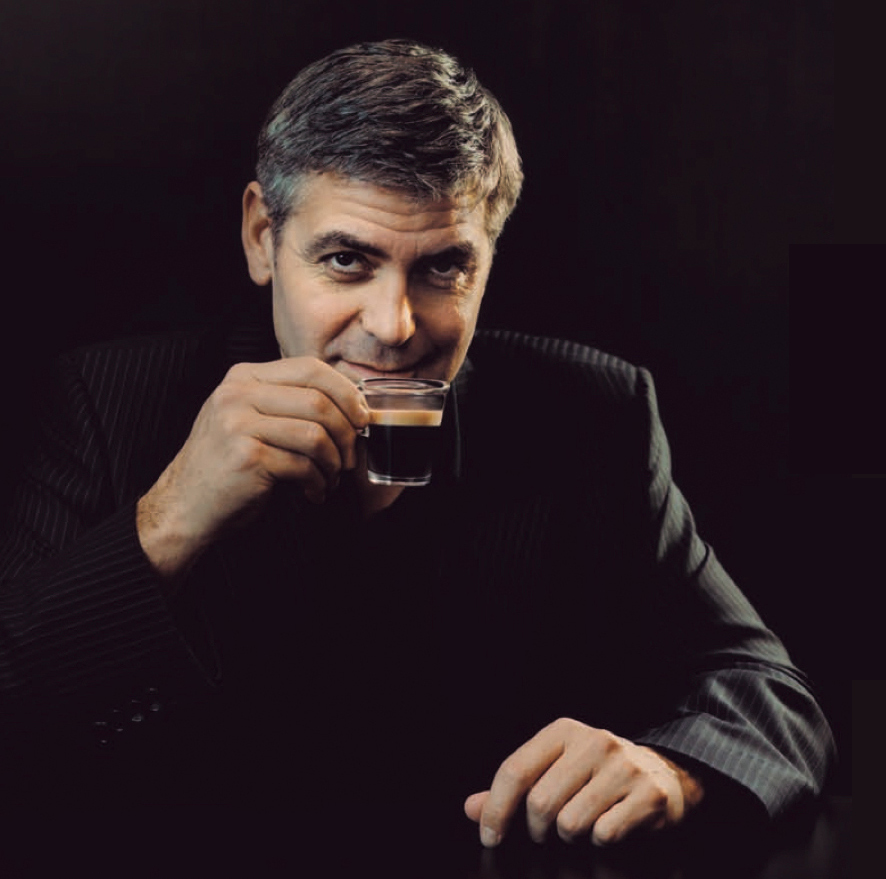
\includegraphics[height=4.0cm]{pics/whatelse.jpg}
    \end{center}

    \pause

    \begin{block}{agent developement is very active}
        \begin{itemize}
            \item code clean up\\
            {\small larger test-suite, modern perl}
            \item architecture changes\\
            {\small event-driven programming, various executable}
            \item smaller memory footprint
        \end{itemize}
    \end{block}
\end{frame}

\begin{frame}
    \frametitle{What else? (2/2)}

    \begin{center}
    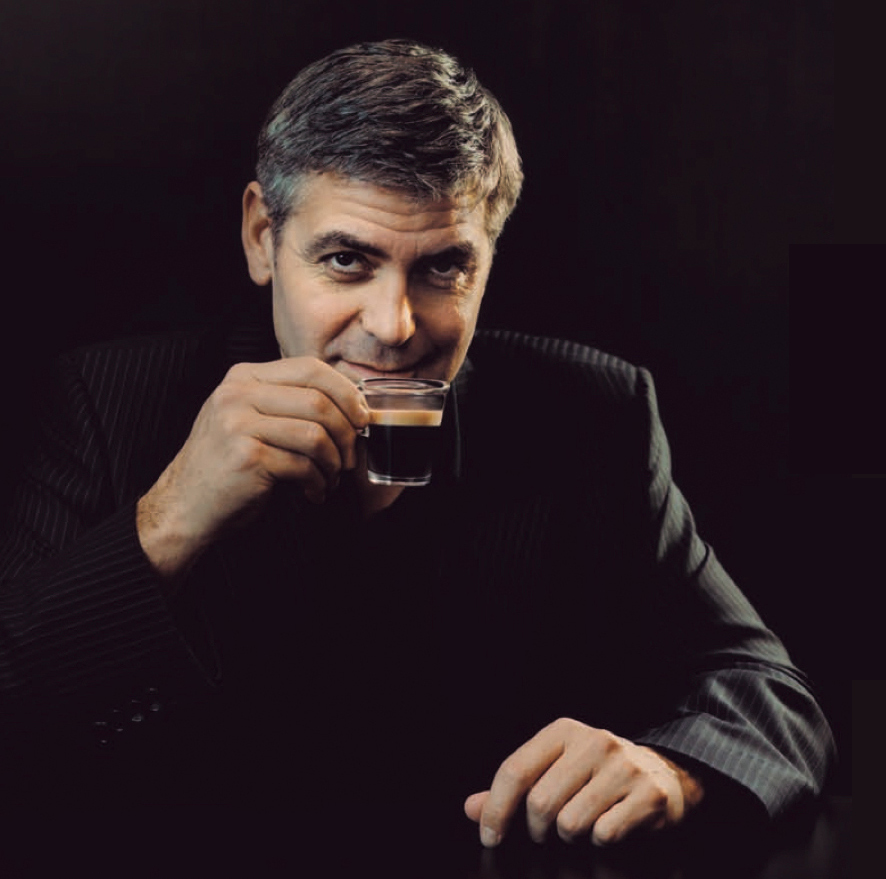
\includegraphics[height=4.0cm]{pics/whatelse.jpg}
    \end{center}

    \begin{block}{In test-suite we trust!}
        \begin{itemize}
            \item strong effort done during the last year \\
            \small{36 800 tests on the GLPI plugin and up to 2 000 on the agent}
            \item with even stronger benefit so far
        \end{itemize}
    \end{block}
\end{frame}

\begin{frame}
    \frametitle{Our roadmap}

    What we are about to release
    \begin{itemize}
    \item FusionInventory for GLPI 0.78: beta planned for this month
    \item ESX inventory: before june
    \item Android Agent
    \end{itemize}

    Work in progress
    \begin{itemize}
    \item Software deployment
    \item OCS/XML → REST/JSON transition
    \end{itemize}
\end{frame}

\begin{frame}
\frametitle{FusionInventory for GLPI 0.78: Action scheduler 1/2}
    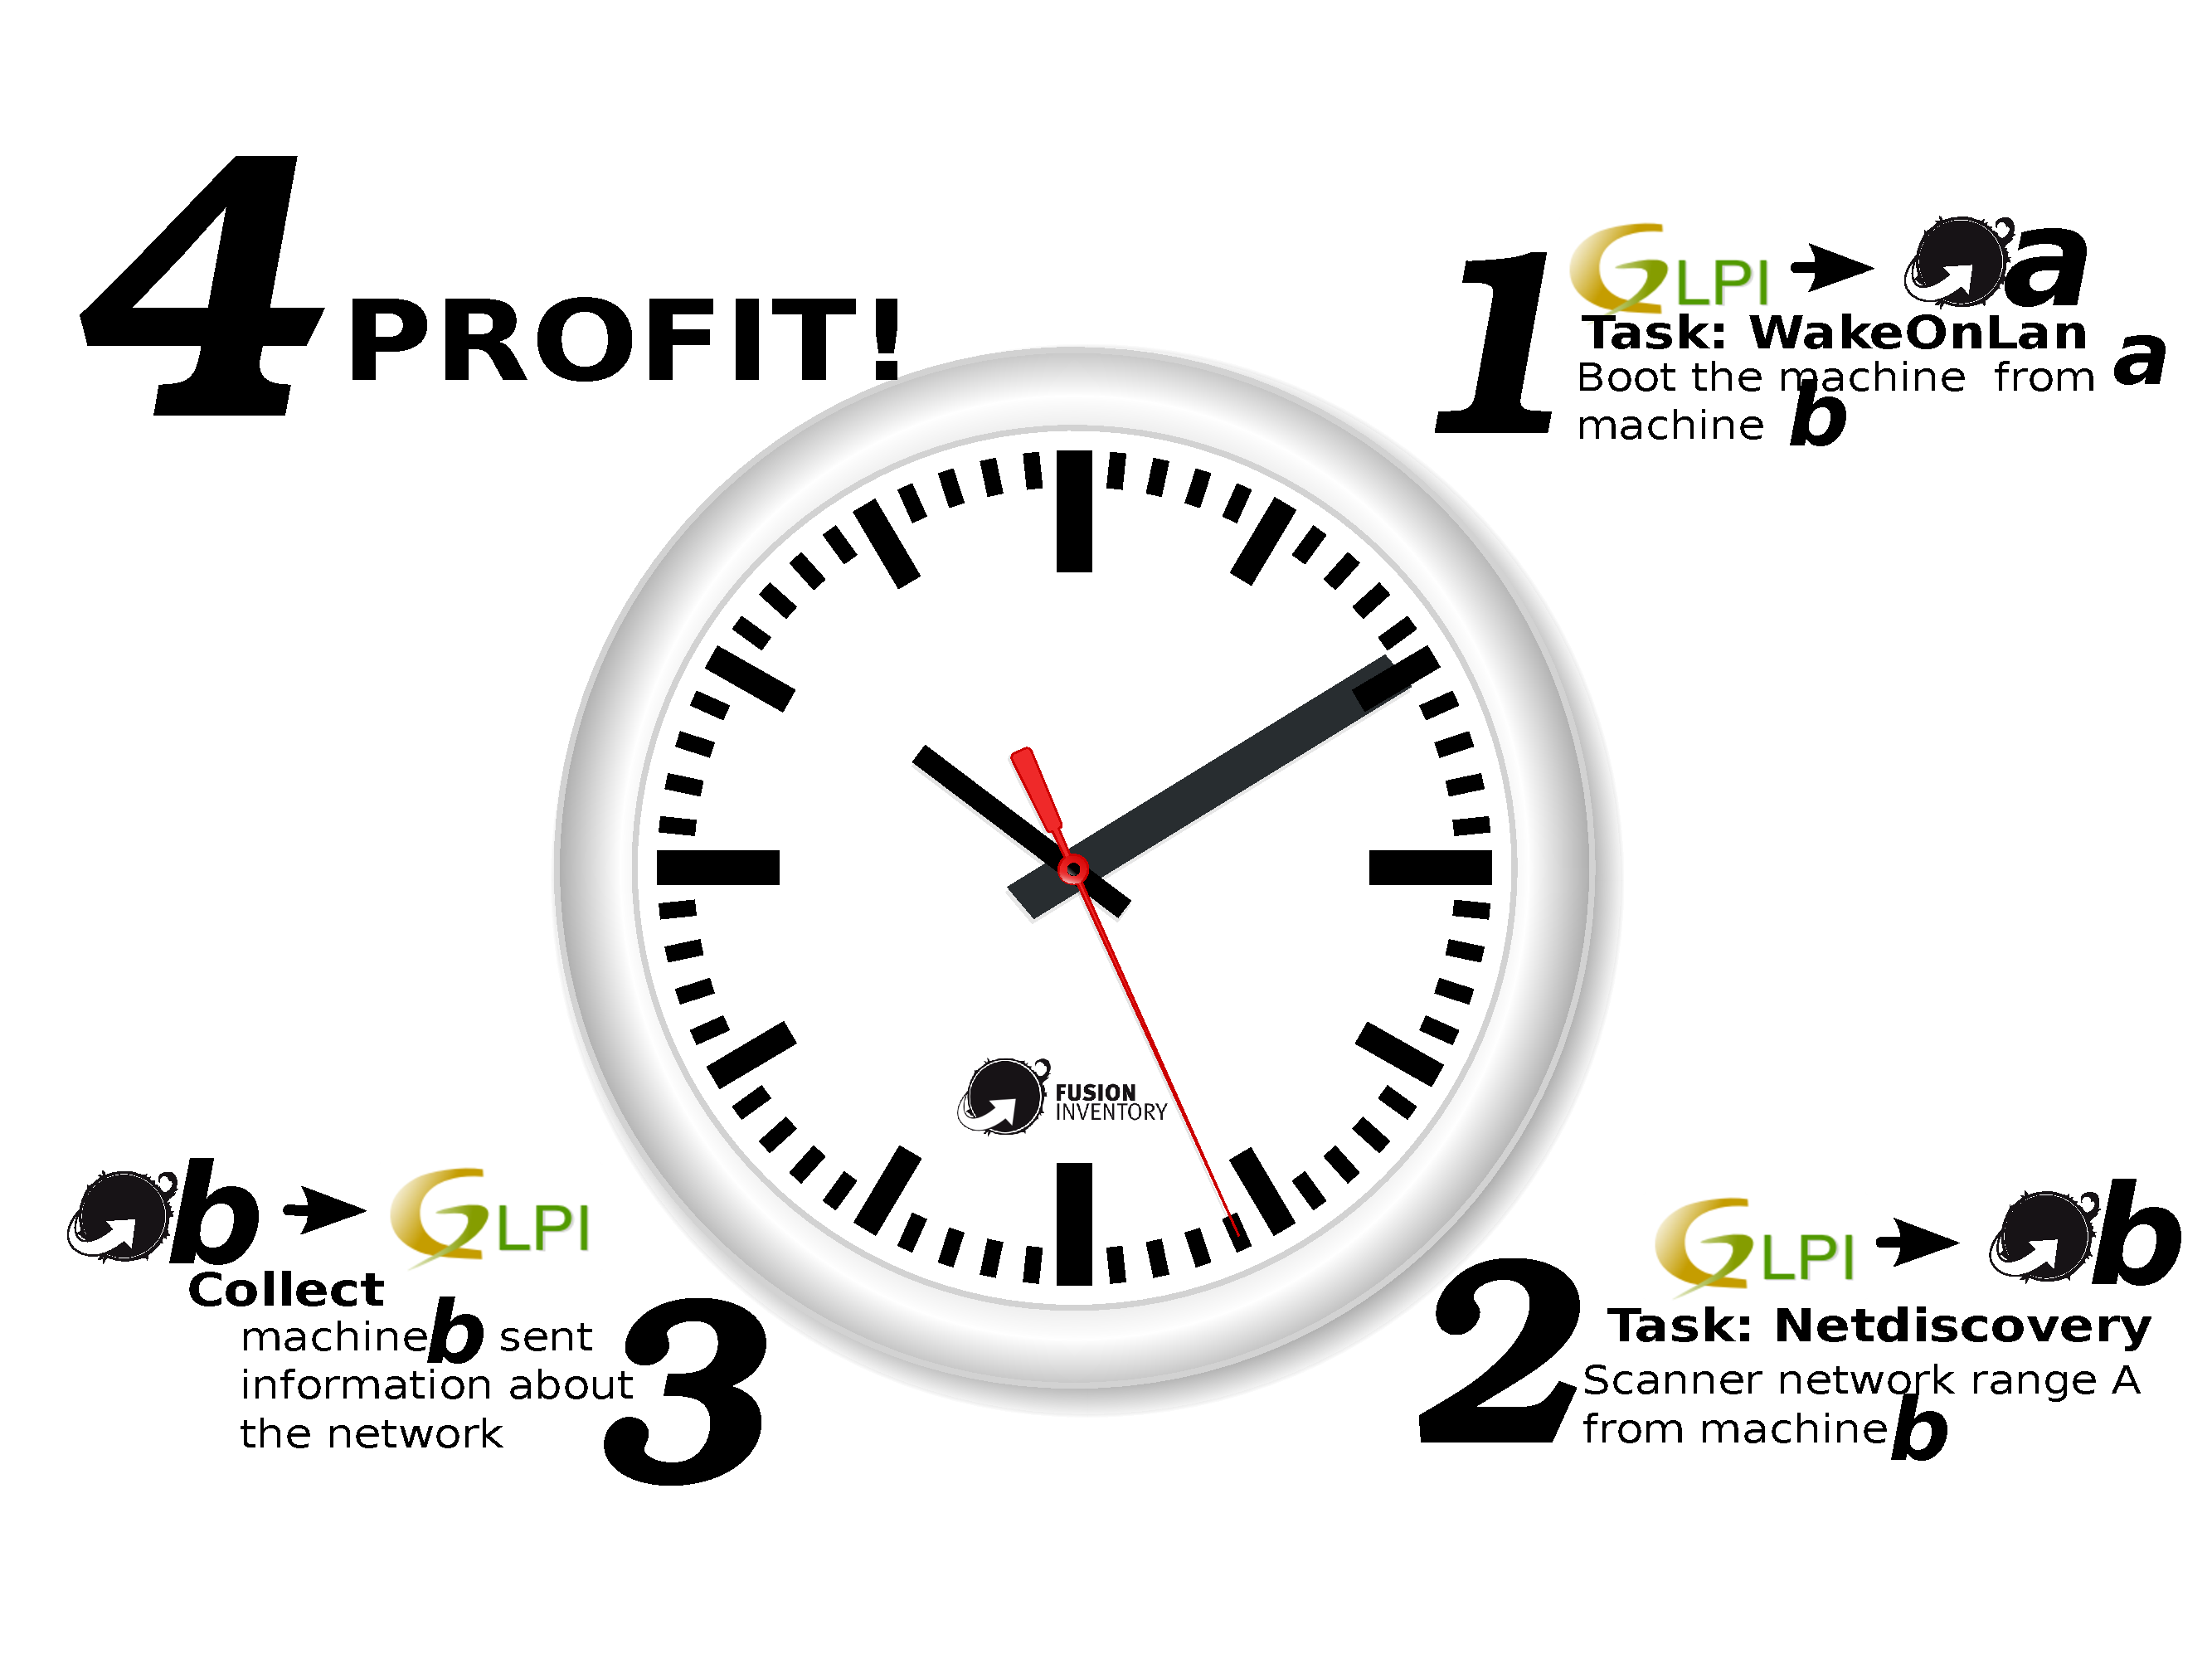
\includegraphics[height=7.5cm]{pics/fusion_task.pdf}
\end{frame}

\begin{frame}
\frametitle{FusionInventory for GLPI 0.78: Action scheduler 2/2}
    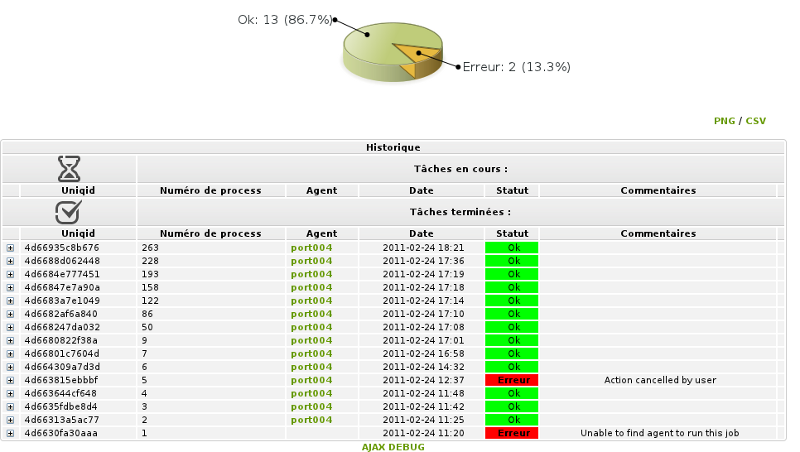
\includegraphics[height=7.5cm]{pics/walid_task_1.png}
\end{frame}

\begin{frame}
\frametitle{FusionInventory for GLPI 0.78: Printer graph}
    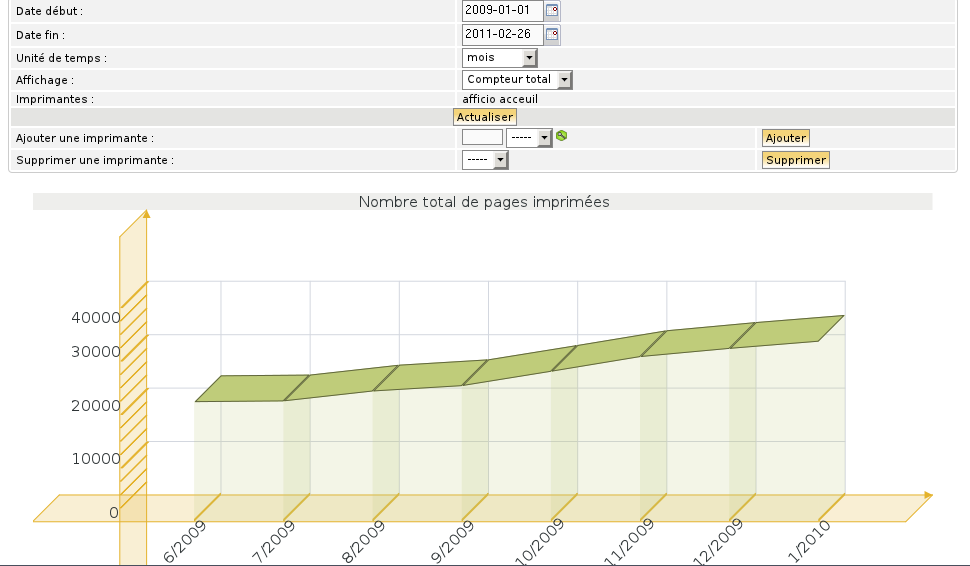
\includegraphics[height=7.5cm]{pics/walid_printer_2.png}
\end{frame}
%



\begin{frame}
\frametitle{ESX 1/2}


   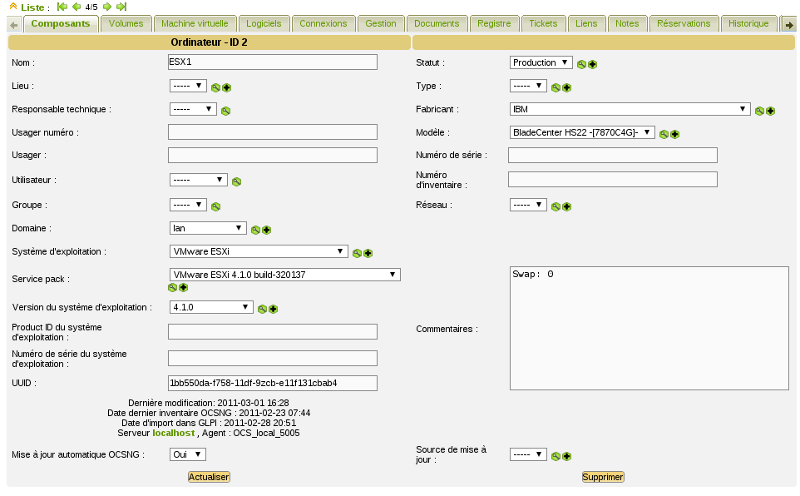
\includegraphics[height=5cm]{./pics/esx1.png}
\end{frame}
%
\begin{frame}
\frametitle{ESX 2/2}


   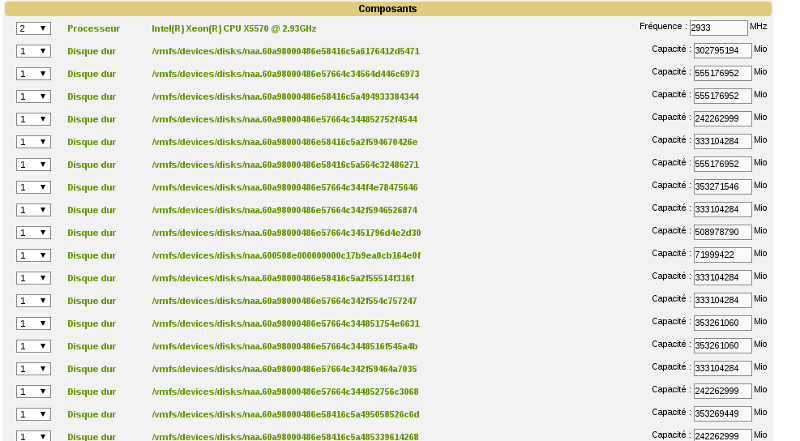
\includegraphics[height=5cm]{./pics/esx2.png}
\end{frame}

%\begin{frame}
%\frametitle{OCS/XML → REST/JSON transition}
%
%\begin{block}{Why}
%    \begin{itemize}
%    \item non standard protocol
%    \begin{itemize}
%    \item unhard to extend: parameters send once whatever you do
%    \item odd XML structure to parse
%    \item hard to extend
%    \end{itemize}
%    \item more modern alternative nowaday
%    \begin{itemize}
%    \item REST
%    \item JSON
%    \end{itemize}
%    \end{itemize}
%\end{block}
%
% \begin{block}{How this will be achieved}
%    \begin{itemize}
%    \item Long transition with dual system
%    \item keep OCS inventory compatibiliy
%    \end{itemize}
%\end{block}

%\end{frame}

\begin{frame}
    \frametitle{Demo}

   
\includegraphics[height=5cm]{./pics/fusinvglpi.png}

    \bf{Demo time!}
\end{frame}


\section{Installation}

\section{Inventory}

\begin{frame}

    \frametitle{The inventories}

    \begin{description}
        \item[BIOS] serial numbers, UUID, ... local
        \item[Memory] memory slot, size, ...
        \item[CPU] frequency, name, manufacturer, ...
        \item[Software] apt-get, yum, Windows software, BSD pkg, ...
        \item[Harddrive] serial number, manufacturer, ...
        \item[Partition] ...
        \item[Virtual Machine] libvirt, xen, ...
        \item[USB devices] phone, USB key, ...
        \item[...] \href{http://search.cpan.org/dist/FusionInventory-Agent/lib/FusionInventory/Agent/XML/Query/Inventory.pm}{see the list on Internet.}
    \end{description}

    It's easy to add new information. Just ask us or submit patches!

\end{frame}



\section{Network Discovery}

\section{SNMP}

\begin{frame}
    \frametitle{SNMP: Goal}

    \begin{itemize}
    \item Identify devices remotly
    \item Inventory devices by SNMP
    \end{itemize}
\end{frame}

\begin{frame}
    \frametitle{SNMP: history}

    \begin{itemize}
    \item Created in 1992
    \item Created for monitoring devices
    \item Some RFC are writen to implement it with standard
    \end{itemize}
\end{frame}

\begin{frame}
    \frametitle{SNMP: Why create own models}

    MIB exists but
    \begin{itemize}
    \item Difficult to find (not for all of course)
    \item MIB not complete
    \item OID not always same on device (depend of model and firmware)
    \end{itemize}
    With models, we are sure device is very nice supported!
\end{frame}

\begin{frame}
    \frametitle{SNMP: What is these models}

    We store these informations
    \begin{itemize}
    \item Relation OID with information (like serial number is oid .1.3...)
    \item Simple or dynamic OID (a serial number or name of each port)
    \end{itemize}

    How to make them?
    \begin{itemize}
    \item We use a complete snmpwalk of each device + model + firmware
    \item Our tool permit to preselect and select OID 
    \item This tool will create and export models 
    \end{itemize}
\end{frame}

\begin{frame}
    \frametitle{SNMP: Switch specification (1/3)}

    Get switch informations 
    \begin{itemize}
    \item Serial number
    \item Manufacturer
    \item Model
    \item Firmware
    \item Mac address    
    \item etc
    \end{itemize}
\end{frame}

\begin{frame}
    \frametitle{SNMP: Switch specification (2/3)}

    Get ports
    \begin{itemize}
    \item Name
    \item Network speed
    \item Port status (enabled / disabled)
    \item Errors input \& output
    \item VLAN
    \item Trunk (tagged)
    \item Active connection
    \end{itemize}
\end{frame}

\begin{frame}
    \frametitle{SNMP: Switch specification (3/3)}

    Get connections on each port
    \begin{itemize}
    \item Mac addresses (one or many on some case)
    \item LLDP \& CDP neighbors (dialog \& informations  between switches)
    \end{itemize}
\end{frame}

\section{Wake On Line}

\section{ESX Inventory}

\section{Questions}

\begin{frame}
    \frametitle{Questions?}

%    \bf{Questions?}
    \begin{center}

    
\includegraphics[height=5cm]{./pics/question.pdf}

    \end{center}
%    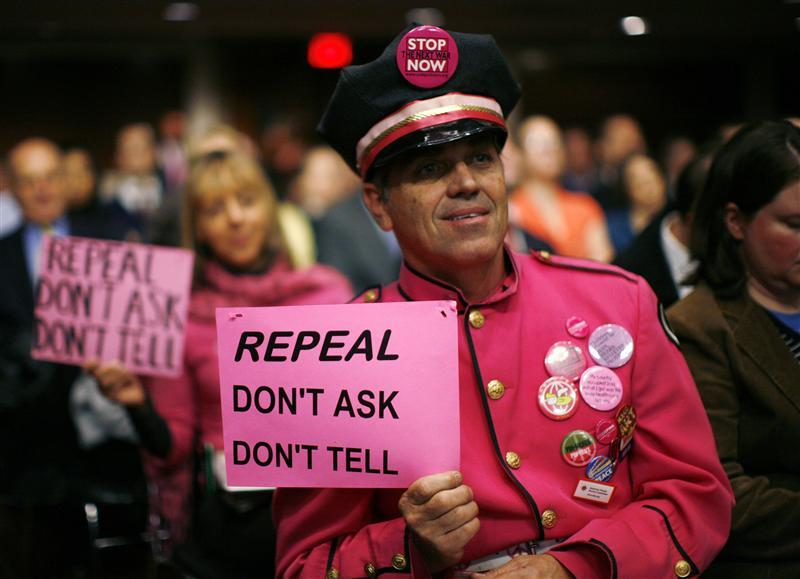
\includegraphics[height=7.5cm]{./pics/ask.jpg}

\end{frame}



\end{document}
